\documentclass[twoside]{book}

% Packages required by doxygen
\usepackage{fixltx2e}
\usepackage{calc}
\usepackage{doxygen}
\usepackage{graphicx}
\usepackage[utf8]{inputenc}
\usepackage{makeidx}
\usepackage{multicol}
\usepackage{multirow}
\PassOptionsToPackage{warn}{textcomp}
\usepackage{textcomp}
\usepackage[nointegrals]{wasysym}
\usepackage[table]{xcolor}
\usepackage{ifpdf,ifxetex}

% Font selection
\usepackage[T1]{fontenc}
\usepackage[scaled=.90]{helvet}
\usepackage{courier}
\usepackage{amssymb}
\usepackage{sectsty}
\renewcommand{\familydefault}{\sfdefault}
\allsectionsfont{%
  \fontseries{bc}\selectfont%
  \color{darkgray}%
}
\renewcommand{\DoxyLabelFont}{%
  \fontseries{bc}\selectfont%
  \color{darkgray}%
}
\newcommand{\+}{\discretionary{\mbox{\scriptsize$\hookleftarrow$}}{}{}}

% Page & text layout
\usepackage{geometry}
\geometry{%
  a4paper,%
  top=2.5cm,%
  bottom=2.5cm,%
  left=2.5cm,%
  right=2.5cm%
}
\tolerance=750
\hfuzz=15pt
\hbadness=750
\setlength{\emergencystretch}{15pt}
\setlength{\parindent}{0cm}
\setlength{\parskip}{3ex plus 2ex minus 2ex}
\makeatletter
\renewcommand{\paragraph}{%
  \@startsection{paragraph}{4}{0ex}{-1.0ex}{1.0ex}{%
    \normalfont\normalsize\bfseries\SS@parafont%
  }%
}
\renewcommand{\subparagraph}{%
  \@startsection{subparagraph}{5}{0ex}{-1.0ex}{1.0ex}{%
    \normalfont\normalsize\bfseries\SS@subparafont%
  }%
}
\makeatother

% Headers & footers
\usepackage{fancyhdr}
\pagestyle{fancyplain}
\fancyhead[LE]{\fancyplain{}{\bfseries\thepage}}
\fancyhead[CE]{\fancyplain{}{}}
\fancyhead[RE]{\fancyplain{}{\bfseries\leftmark}}
\fancyhead[LO]{\fancyplain{}{\bfseries\rightmark}}
\fancyhead[CO]{\fancyplain{}{}}
\fancyhead[RO]{\fancyplain{}{\bfseries\thepage}}
\fancyfoot[LE]{\fancyplain{}{}}
\fancyfoot[CE]{\fancyplain{}{}}
\fancyfoot[RE]{\fancyplain{}{\bfseries\scriptsize Generated by Doxygen }}
\fancyfoot[LO]{\fancyplain{}{\bfseries\scriptsize Generated by Doxygen }}
\fancyfoot[CO]{\fancyplain{}{}}
\fancyfoot[RO]{\fancyplain{}{}}
\renewcommand{\footrulewidth}{0.4pt}
\renewcommand{\chaptermark}[1]{%
  \markboth{#1}{}%
}
\renewcommand{\sectionmark}[1]{%
  \markright{\thesection\ #1}%
}

% Indices & bibliography
\usepackage{natbib}
\usepackage[titles]{tocloft}
\setcounter{tocdepth}{3}
\setcounter{secnumdepth}{5}
\makeindex

% Hyperlinks (required, but should be loaded last)
\ifpdf
  \usepackage[pdftex,pagebackref=true]{hyperref}
\else
  \ifxetex
    \usepackage[pagebackref=true]{hyperref}
  \else
    \usepackage[ps2pdf,pagebackref=true]{hyperref}
  \fi
\fi
\ifpdf
  \DeclareUnicodeCharacter{207B}{${}^{-}$}% Superscript minus
  \DeclareUnicodeCharacter{C2B2}{${}^{2}$}% Superscript two
  \DeclareUnicodeCharacter{C2B3}{${}^{3}$}% Superscript three
\else
  \catcode`\⁻=13% Superscript minus
  \def⁻{${}^{-}$}
  \catcode`\²=13% Superscript two
  \def²{${}^{2}$}
  \catcode`\³=13% Superscript three
  \def³{${}^{3}$}
\fi

\hypersetup{%
  colorlinks=true,%
  linkcolor=blue,%
  citecolor=blue,%
  unicode%
}

% Custom commands
\newcommand{\clearemptydoublepage}{%
  \newpage{\pagestyle{empty}\cleardoublepage}%
}

\usepackage{caption}
\captionsetup{labelsep=space,justification=centering,font={bf},singlelinecheck=off,skip=4pt,position=top}

\renewcommand{\numberline}[1]{#1~}
%===== C O N T E N T S =====

\begin{document}

% Titlepage & ToC
\hypersetup{pageanchor=false,
             bookmarksnumbered=true,
             pdfencoding=unicode
            }
\pagenumbering{alph}
\begin{titlepage}
\vspace*{7cm}
\begin{center}%
{\Large Spellcheck }\\
\vspace*{1cm}
{\large Generated by Doxygen 1.8.15}\\
\end{center}
\end{titlepage}
\clearemptydoublepage
\pagenumbering{roman}
\tableofcontents
\clearemptydoublepage
\pagenumbering{arabic}
\hypersetup{pageanchor=true}

%--- Begin generated contents ---
\chapter{Hierarchical Index}
\section{Class Hierarchy}
This inheritance list is sorted roughly, but not completely, alphabetically\+:\begin{DoxyCompactList}
\item \contentsline{section}{config}{\pageref{structconfig}}{}
\item \contentsline{section}{dict}{\pageref{structdict}}{}
\item \contentsline{section}{dict\+\_\+t}{\pageref{structdict__t}}{}
\item \contentsline{section}{dict\+Entry}{\pageref{structdict_entry}}{}
\item \contentsline{section}{dict\+Iterator}{\pageref{structdict_iterator}}{}
\item \contentsline{section}{dict\+Type}{\pageref{structdict_type}}{}
\item \contentsline{section}{match\+\_\+t}{\pageref{structmatch__t}}{}
\item Q\+Object\begin{DoxyCompactList}
\item \contentsline{section}{Example\+Qt}{\pageref{class_example_qt}}{}
\item \contentsline{section}{Redis\+Qt\+Adapter}{\pageref{class_redis_qt_adapter}}{}
\end{DoxyCompactList}
\item \contentsline{section}{redis\+Ae\+Events}{\pageref{structredis_ae_events}}{}
\item \contentsline{section}{redis\+Async\+Context}{\pageref{structredis_async_context}}{}
\item \contentsline{section}{redis\+Callback}{\pageref{structredis_callback}}{}
\item \contentsline{section}{redis\+Callback\+List}{\pageref{structredis_callback_list}}{}
\item \contentsline{section}{redis\+Context}{\pageref{structredis_context}}{}
\item \contentsline{section}{redis\+Ivykis\+Events}{\pageref{structredis_ivykis_events}}{}
\item \contentsline{section}{redis\+Libevent\+Events}{\pageref{structredis_libevent_events}}{}
\item \contentsline{section}{redis\+Libev\+Events}{\pageref{structredis_libev_events}}{}
\item \contentsline{section}{redis\+Libuv\+Events}{\pageref{structredis_libuv_events}}{}
\item \contentsline{section}{redis\+Reader}{\pageref{structredis_reader}}{}
\item \contentsline{section}{redis\+Read\+Task}{\pageref{structredis_read_task}}{}
\item \contentsline{section}{redis\+Reply}{\pageref{structredis_reply}}{}
\item \contentsline{section}{redis\+Reply\+Object\+Functions}{\pageref{structredis_reply_object_functions}}{}
\item \contentsline{section}{Redis\+Run\+Loop}{\pageref{struct_redis_run_loop}}{}
\item \contentsline{section}{Redis\+Source}{\pageref{struct_redis_source}}{}
\item \contentsline{section}{sdshdr}{\pageref{structsdshdr}}{}
\item \contentsline{section}{trie}{\pageref{structtrie}}{}
\item \contentsline{section}{trie\+\_\+t}{\pageref{structtrie__t}}{}
\item \contentsline{section}{zset\+\_\+t}{\pageref{structzset__t}}{}
\end{DoxyCompactList}

\chapter{Class Index}
\section{Class List}
Here are the classes, structs, unions and interfaces with brief descriptions\+:\begin{DoxyCompactList}
\item\contentsline{section}{\mbox{\hyperlink{structdict__t}{dict\+\_\+t}} \\*A dictionary and a instant lookup table of the characters contained in it }{\pageref{structdict__t}}{}
\end{DoxyCompactList}

\chapter{File Index}
\section{File List}
Here is a list of all documented files with brief descriptions\+:\begin{DoxyCompactList}
\item\contentsline{section}{/\+Users/jaewanpark/\+Desktop/\+V\+M\+\_\+\+R\+E\+P\+O\+\_\+\+R\+O\+O\+T/spellcheck/include/\mbox{\hyperlink{dictionary_8h}{dictionary.\+h}} }{\pageref{dictionary_8h}}{}
\item\contentsline{section}{/\+Users/jaewanpark/\+Desktop/\+V\+M\+\_\+\+R\+E\+P\+O\+\_\+\+R\+O\+O\+T/spellcheck/include/\mbox{\hyperlink{main__functions__batch_8h}{main\+\_\+functions\+\_\+batch.\+h}} }{\pageref{main__functions__batch_8h}}{}
\item\contentsline{section}{/\+Users/jaewanpark/\+Desktop/\+V\+M\+\_\+\+R\+E\+P\+O\+\_\+\+R\+O\+O\+T/spellcheck/include/\mbox{\hyperlink{main__functions__edit_8h}{main\+\_\+functions\+\_\+edit.\+h}} }{\pageref{main__functions__edit_8h}}{}
\item\contentsline{section}{/\+Users/jaewanpark/\+Desktop/\+V\+M\+\_\+\+R\+E\+P\+O\+\_\+\+R\+O\+O\+T/spellcheck/include/\mbox{\hyperlink{main__functions__home_8h}{main\+\_\+functions\+\_\+home.\+h}} }{\pageref{main__functions__home_8h}}{}
\item\contentsline{section}{/\+Users/jaewanpark/\+Desktop/\+V\+M\+\_\+\+R\+E\+P\+O\+\_\+\+R\+O\+O\+T/spellcheck/include/\mbox{\hyperlink{main__functions__interactive_8h}{main\+\_\+functions\+\_\+interactive.\+h}} }{\pageref{main__functions__interactive_8h}}{}
\item\contentsline{section}{/\+Users/jaewanpark/\+Desktop/\+V\+M\+\_\+\+R\+E\+P\+O\+\_\+\+R\+O\+O\+T/spellcheck/include/\mbox{\hyperlink{main__functions__save_8h}{main\+\_\+functions\+\_\+save.\+h}} }{\pageref{main__functions__save_8h}}{}
\item\contentsline{section}{/\+Users/jaewanpark/\+Desktop/\+V\+M\+\_\+\+R\+E\+P\+O\+\_\+\+R\+O\+O\+T/spellcheck/include/\mbox{\hyperlink{parser_8h}{parser.\+h}} }{\pageref{parser_8h}}{}
\item\contentsline{section}{/\+Users/jaewanpark/\+Desktop/\+V\+M\+\_\+\+R\+E\+P\+O\+\_\+\+R\+O\+O\+T/spellcheck/include/\mbox{\hyperlink{shellstrings_8h}{shellstrings.\+h}} }{\pageref{shellstrings_8h}}{}
\item\contentsline{section}{/\+Users/jaewanpark/\+Desktop/\+V\+M\+\_\+\+R\+E\+P\+O\+\_\+\+R\+O\+O\+T/spellcheck/include/\mbox{\hyperlink{word_8h}{word.\+h}} }{\pageref{word_8h}}{}
\end{DoxyCompactList}

\chapter{Class Documentation}
\hypertarget{structconfig}{}\section{config Struct Reference}
\label{structconfig}\index{config@{config}}
\subsection*{Public Attributes}
\begin{DoxyCompactItemize}
\item 
\mbox{\Hypertarget{structconfig_ac1a4369bee218f0b8bee7d9d3c35e0ca}\label{structconfig_ac1a4369bee218f0b8bee7d9d3c35e0ca}} 
enum connection\+\_\+type {\bfseries type}
\item 
\mbox{\Hypertarget{structconfig_a12dd2ad802175c54411ee3e02832f27f}\label{structconfig_a12dd2ad802175c54411ee3e02832f27f}} 
\begin{tabbing}
xx\=xx\=xx\=xx\=xx\=xx\=xx\=xx\=xx\=\kill
struct \{\\
\>const char $\ast$ {\bfseries host}\\
\>int {\bfseries port}\\
\>struct timeval {\bfseries timeout}\\
\} {\bfseries tcp}\\

\end{tabbing}\item 
\mbox{\Hypertarget{structconfig_a9d30f10a9246c20451418e5756926bdb}\label{structconfig_a9d30f10a9246c20451418e5756926bdb}} 
\begin{tabbing}
xx\=xx\=xx\=xx\=xx\=xx\=xx\=xx\=xx\=\kill
struct \{\\
\>const char $\ast$ {\bfseries path}\\
\} {\bfseries unix}\\

\end{tabbing}\end{DoxyCompactItemize}


The documentation for this struct was generated from the following file\+:\begin{DoxyCompactItemize}
\item 
/\+Users/firatciftci/spellcheck/api/lib/hiredis-\/0.\+13.\+3/test.\+c\end{DoxyCompactItemize}

\hypertarget{structdict}{}\section{dict Struct Reference}
\label{structdict}\index{dict@{dict}}
\subsection*{Public Attributes}
\begin{DoxyCompactItemize}
\item 
\mbox{\Hypertarget{structdict_a22d4788abe9d2d3ee5232d0b22fb13a5}\label{structdict_a22d4788abe9d2d3ee5232d0b22fb13a5}} 
\mbox{\hyperlink{structdict_entry}{dict\+Entry}} $\ast$$\ast$ {\bfseries table}
\item 
\mbox{\Hypertarget{structdict_a89da3d5d54bd930937587a3c411af5fd}\label{structdict_a89da3d5d54bd930937587a3c411af5fd}} 
\mbox{\hyperlink{structdict_type}{dict\+Type}} $\ast$ {\bfseries type}
\item 
\mbox{\Hypertarget{structdict_a296b58c7e6078a0dd8077e1432ac58b4}\label{structdict_a296b58c7e6078a0dd8077e1432ac58b4}} 
unsigned long {\bfseries size}
\item 
\mbox{\Hypertarget{structdict_ac948fbd3c50396124dad4e3a26431043}\label{structdict_ac948fbd3c50396124dad4e3a26431043}} 
unsigned long {\bfseries sizemask}
\item 
\mbox{\Hypertarget{structdict_a99eb5e81eea744d77d84dc591e7cecca}\label{structdict_a99eb5e81eea744d77d84dc591e7cecca}} 
unsigned long {\bfseries used}
\item 
\mbox{\Hypertarget{structdict_a36ce9f4e7d035fa4d7d2886f30b6a9af}\label{structdict_a36ce9f4e7d035fa4d7d2886f30b6a9af}} 
void $\ast$ {\bfseries privdata}
\end{DoxyCompactItemize}


The documentation for this struct was generated from the following file\+:\begin{DoxyCompactItemize}
\item 
/\+Users/firatciftci/spellcheck/api/lib/hiredis-\/0.\+13.\+3/dict.\+h\end{DoxyCompactItemize}

\hypertarget{structdict__t}{}\section{dict\+\_\+t Struct Reference}
\label{structdict__t}\index{dict\+\_\+t@{dict\+\_\+t}}


A dictionary and a instant lookup table of the characters contained in it.  




{\ttfamily \#include $<$dictionary.\+h$>$}

\subsection*{Public Member Functions}
\begin{DoxyCompactItemize}
\item 
\mbox{\hyperlink{structdict__t}{dict\+\_\+t}} $\ast$ \mbox{\hyperlink{structdict__t_a0074913fdba65680670bf93153225e2f}{dict\+\_\+new}} ()
\begin{DoxyCompactList}\small\item\em Allocates a new dictionary. \end{DoxyCompactList}\item 
int \mbox{\hyperlink{structdict__t_a81c807e5c6b67b7b482dcac658c0fc57}{dict\+\_\+init}} (\mbox{\hyperlink{structdict__t}{dict\+\_\+t}} $\ast$d)
\begin{DoxyCompactList}\small\item\em Initializes a dictionary. \end{DoxyCompactList}\item 
int \mbox{\hyperlink{structdict__t_a51ee6c067decce8dbc182f95f7b33e91}{dict\+\_\+free}} (\mbox{\hyperlink{structdict__t}{dict\+\_\+t}} $\ast$d)
\begin{DoxyCompactList}\small\item\em Frees the resources associated with a dictionary. \end{DoxyCompactList}\item 
int \mbox{\hyperlink{structdict__t_acc7f38511d6fbf572b62e2aeac7ffddc}{dict\+\_\+chars\+\_\+exists}} (\mbox{\hyperlink{structdict__t}{dict\+\_\+t}} $\ast$d, char c)
\begin{DoxyCompactList}\small\item\em Returns whether a character is in the character list. \end{DoxyCompactList}\item 
int \mbox{\hyperlink{structdict__t_afb48275334e47ae9cab20e1837f0bbcf}{dict\+\_\+chars\+\_\+update}} (\mbox{\hyperlink{structdict__t}{dict\+\_\+t}} $\ast$d, char $\ast$str)
\begin{DoxyCompactList}\small\item\em Updates the character list with potential new characters from a string. \end{DoxyCompactList}\item 
int \mbox{\hyperlink{structdict__t_ada2e9cd98e98ccefe871124833a4cd77}{dict\+\_\+exists}} (\mbox{\hyperlink{structdict__t}{dict\+\_\+t}} $\ast$d, char $\ast$str)
\begin{DoxyCompactList}\small\item\em Checks if a string is contained in a dictionary. \end{DoxyCompactList}\item 
int \mbox{\hyperlink{structdict__t_ab4825a90819a79433cd1f4f6034b4fc1}{dict\+\_\+add}} (\mbox{\hyperlink{structdict__t}{dict\+\_\+t}} $\ast$d, char $\ast$str)
\begin{DoxyCompactList}\small\item\em Adds a word to a dictionary. \end{DoxyCompactList}\item 
int \mbox{\hyperlink{structdict__t_a4a2d3fd1ef3eba7b6e70d87129ad347f}{dict\+\_\+read}} (\mbox{\hyperlink{structdict__t}{dict\+\_\+t}} $\ast$d, char $\ast$file)
\begin{DoxyCompactList}\small\item\em Parses a file and adds all words to the dictionary. \end{DoxyCompactList}\item 
char $\ast$$\ast$ \mbox{\hyperlink{structdict__t_af7a2a46644a6279d42ddda31bfde70e2}{dict\+\_\+suggestions}} (\mbox{\hyperlink{structdict__t}{dict\+\_\+t}} $\ast$d, char $\ast$str, int max\+\_\+edits, int n)
\begin{DoxyCompactList}\small\item\em Returns the n closest words to a given string in a dictionary. \end{DoxyCompactList}\end{DoxyCompactItemize}
\subsection*{Public Attributes}
\begin{DoxyCompactItemize}
\item 
\mbox{\Hypertarget{structdict__t_a4743f4cde2360543d7976d68e0bfacee}\label{structdict__t_a4743f4cde2360543d7976d68e0bfacee}} 
trie\+\_\+t $\ast$ {\bfseries dict}
\end{DoxyCompactItemize}


\subsection{Detailed Description}
A dictionary and a instant lookup table of the characters contained in it. 

\subsection{Member Function Documentation}
\mbox{\Hypertarget{structdict__t_ab4825a90819a79433cd1f4f6034b4fc1}\label{structdict__t_ab4825a90819a79433cd1f4f6034b4fc1}} 
\index{dict\+\_\+t@{dict\+\_\+t}!dict\+\_\+add@{dict\+\_\+add}}
\index{dict\+\_\+add@{dict\+\_\+add}!dict\+\_\+t@{dict\+\_\+t}}
\subsubsection{\texorpdfstring{dict\+\_\+add()}{dict\_add()}}
{\footnotesize\ttfamily int dict\+\_\+add (\begin{DoxyParamCaption}\item[{\mbox{\hyperlink{structdict__t}{dict\+\_\+t}} $\ast$}]{d,  }\item[{char $\ast$}]{str }\end{DoxyParamCaption})}



Adds a word to a dictionary. 


\begin{DoxyParams}{Parameters}
{\em d} & A dictionary. Must point to a dictionary allocated with \mbox{\hyperlink{structdict__t_a0074913fdba65680670bf93153225e2f}{dict\+\_\+new()}}. \\
\hline
{\em str} & A string. \\
\hline
\end{DoxyParams}
\begin{DoxyReturn}{Returns}
E\+X\+I\+T\+\_\+\+S\+U\+C\+C\+E\+SS upon success, E\+X\+I\+T\+\_\+\+F\+A\+I\+L\+U\+RE if word is already in dictionary or if an error occured. 
\end{DoxyReturn}
\mbox{\Hypertarget{structdict__t_acc7f38511d6fbf572b62e2aeac7ffddc}\label{structdict__t_acc7f38511d6fbf572b62e2aeac7ffddc}} 
\index{dict\+\_\+t@{dict\+\_\+t}!dict\+\_\+chars\+\_\+exists@{dict\+\_\+chars\+\_\+exists}}
\index{dict\+\_\+chars\+\_\+exists@{dict\+\_\+chars\+\_\+exists}!dict\+\_\+t@{dict\+\_\+t}}
\subsubsection{\texorpdfstring{dict\+\_\+chars\+\_\+exists()}{dict\_chars\_exists()}}
{\footnotesize\ttfamily int dict\+\_\+chars\+\_\+exists (\begin{DoxyParamCaption}\item[{\mbox{\hyperlink{structdict__t}{dict\+\_\+t}} $\ast$}]{d,  }\item[{char}]{c }\end{DoxyParamCaption})}



Returns whether a character is in the character list. 


\begin{DoxyParams}{Parameters}
{\em d} & A dictionary. Must point to a dictionary allocated with \mbox{\hyperlink{structdict__t_a0074913fdba65680670bf93153225e2f}{dict\+\_\+new()}}. \\
\hline
{\em c} & A character. \\
\hline
\end{DoxyParams}
\begin{DoxyReturn}{Returns}
E\+X\+I\+T\+\_\+\+S\+U\+C\+C\+E\+SS if the character is contained in the dictionary, E\+X\+I\+T\+\_\+\+F\+A\+I\+L\+U\+RE if it isn\textquotesingle{}t. 
\end{DoxyReturn}
\mbox{\Hypertarget{structdict__t_afb48275334e47ae9cab20e1837f0bbcf}\label{structdict__t_afb48275334e47ae9cab20e1837f0bbcf}} 
\index{dict\+\_\+t@{dict\+\_\+t}!dict\+\_\+chars\+\_\+update@{dict\+\_\+chars\+\_\+update}}
\index{dict\+\_\+chars\+\_\+update@{dict\+\_\+chars\+\_\+update}!dict\+\_\+t@{dict\+\_\+t}}
\subsubsection{\texorpdfstring{dict\+\_\+chars\+\_\+update()}{dict\_chars\_update()}}
{\footnotesize\ttfamily int dict\+\_\+chars\+\_\+update (\begin{DoxyParamCaption}\item[{\mbox{\hyperlink{structdict__t}{dict\+\_\+t}} $\ast$}]{d,  }\item[{char $\ast$}]{str }\end{DoxyParamCaption})}



Updates the character list with potential new characters from a string. 


\begin{DoxyParams}{Parameters}
{\em d} & A dictionary. Must point to a dictionary allocated with \mbox{\hyperlink{structdict__t_a0074913fdba65680670bf93153225e2f}{dict\+\_\+new()}}. \\
\hline
{\em str} & A string. \\
\hline
\end{DoxyParams}
\begin{DoxyReturn}{Returns}
E\+X\+I\+T\+\_\+\+S\+U\+C\+C\+E\+SS on success, E\+X\+I\+T\+\_\+\+F\+A\+I\+L\+U\+RE if an error occurs. 
\end{DoxyReturn}
\mbox{\Hypertarget{structdict__t_ada2e9cd98e98ccefe871124833a4cd77}\label{structdict__t_ada2e9cd98e98ccefe871124833a4cd77}} 
\index{dict\+\_\+t@{dict\+\_\+t}!dict\+\_\+exists@{dict\+\_\+exists}}
\index{dict\+\_\+exists@{dict\+\_\+exists}!dict\+\_\+t@{dict\+\_\+t}}
\subsubsection{\texorpdfstring{dict\+\_\+exists()}{dict\_exists()}}
{\footnotesize\ttfamily int dict\+\_\+exists (\begin{DoxyParamCaption}\item[{\mbox{\hyperlink{structdict__t}{dict\+\_\+t}} $\ast$}]{d,  }\item[{char $\ast$}]{str }\end{DoxyParamCaption})}



Checks if a string is contained in a dictionary. 


\begin{DoxyParams}{Parameters}
{\em d} & A dictionary. Must point to a dictionary allocated with \mbox{\hyperlink{structdict__t_a0074913fdba65680670bf93153225e2f}{dict\+\_\+new()}}. \\
\hline
{\em str} & A string. \\
\hline
\end{DoxyParams}
\begin{DoxyReturn}{Returns}
E\+X\+I\+T\+\_\+\+S\+U\+C\+C\+E\+SS if the word is in the dictionary, E\+X\+I\+T\+\_\+\+F\+A\+I\+L\+U\+RE if the word is not in the dictionary or if an error occured. 
\end{DoxyReturn}
\mbox{\Hypertarget{structdict__t_a51ee6c067decce8dbc182f95f7b33e91}\label{structdict__t_a51ee6c067decce8dbc182f95f7b33e91}} 
\index{dict\+\_\+t@{dict\+\_\+t}!dict\+\_\+free@{dict\+\_\+free}}
\index{dict\+\_\+free@{dict\+\_\+free}!dict\+\_\+t@{dict\+\_\+t}}
\subsubsection{\texorpdfstring{dict\+\_\+free()}{dict\_free()}}
{\footnotesize\ttfamily int dict\+\_\+free (\begin{DoxyParamCaption}\item[{\mbox{\hyperlink{structdict__t}{dict\+\_\+t}} $\ast$}]{d }\end{DoxyParamCaption})}



Frees the resources associated with a dictionary. 


\begin{DoxyParams}{Parameters}
{\em d} & A dictionary. Must point to a dictionary allocated with \mbox{\hyperlink{structdict__t_a0074913fdba65680670bf93153225e2f}{dict\+\_\+new()}}. \\
\hline
\end{DoxyParams}
\begin{DoxyReturn}{Returns}
Always returns E\+X\+I\+T\+\_\+\+S\+U\+C\+C\+E\+SS. 
\end{DoxyReturn}
\mbox{\Hypertarget{structdict__t_a81c807e5c6b67b7b482dcac658c0fc57}\label{structdict__t_a81c807e5c6b67b7b482dcac658c0fc57}} 
\index{dict\+\_\+t@{dict\+\_\+t}!dict\+\_\+init@{dict\+\_\+init}}
\index{dict\+\_\+init@{dict\+\_\+init}!dict\+\_\+t@{dict\+\_\+t}}
\subsubsection{\texorpdfstring{dict\+\_\+init()}{dict\_init()}}
{\footnotesize\ttfamily int dict\+\_\+init (\begin{DoxyParamCaption}\item[{\mbox{\hyperlink{structdict__t}{dict\+\_\+t}} $\ast$}]{d }\end{DoxyParamCaption})}



Initializes a dictionary. 


\begin{DoxyParams}{Parameters}
{\em d} & A dictionary. Must point to a dictionary allocated with \mbox{\hyperlink{structdict__t_a0074913fdba65680670bf93153225e2f}{dict\+\_\+new()}}. \\
\hline
\end{DoxyParams}
\begin{DoxyReturn}{Returns}
E\+X\+I\+T\+\_\+\+S\+U\+C\+C\+E\+SS on success, E\+X\+I\+T\+\_\+\+F\+A\+I\+L\+U\+RE if an error occurs. 
\end{DoxyReturn}
\mbox{\Hypertarget{structdict__t_a0074913fdba65680670bf93153225e2f}\label{structdict__t_a0074913fdba65680670bf93153225e2f}} 
\index{dict\+\_\+t@{dict\+\_\+t}!dict\+\_\+new@{dict\+\_\+new}}
\index{dict\+\_\+new@{dict\+\_\+new}!dict\+\_\+t@{dict\+\_\+t}}
\subsubsection{\texorpdfstring{dict\+\_\+new()}{dict\_new()}}
{\footnotesize\ttfamily \mbox{\hyperlink{structdict__t}{dict\+\_\+t}} $\ast$ dict\+\_\+new (\begin{DoxyParamCaption}{ }\end{DoxyParamCaption})}



Allocates a new dictionary. 

\begin{DoxyReturn}{Returns}
A pointer to the dictionary, or N\+U\+LL if a dictionary cannot be allocated. 
\end{DoxyReturn}
\mbox{\Hypertarget{structdict__t_a4a2d3fd1ef3eba7b6e70d87129ad347f}\label{structdict__t_a4a2d3fd1ef3eba7b6e70d87129ad347f}} 
\index{dict\+\_\+t@{dict\+\_\+t}!dict\+\_\+read@{dict\+\_\+read}}
\index{dict\+\_\+read@{dict\+\_\+read}!dict\+\_\+t@{dict\+\_\+t}}
\subsubsection{\texorpdfstring{dict\+\_\+read()}{dict\_read()}}
{\footnotesize\ttfamily int dict\+\_\+read (\begin{DoxyParamCaption}\item[{\mbox{\hyperlink{structdict__t}{dict\+\_\+t}} $\ast$}]{d,  }\item[{char $\ast$}]{file }\end{DoxyParamCaption})}



Parses a file and adds all words to the dictionary. 


\begin{DoxyParams}{Parameters}
{\em d} & A dictionary. Must point to a dictionary allocated with \mbox{\hyperlink{structdict__t_a0074913fdba65680670bf93153225e2f}{dict\+\_\+new()}}. \\
\hline
{\em file} & File being input. \\
\hline
\end{DoxyParams}
\begin{DoxyReturn}{Returns}
E\+X\+I\+T\+\_\+\+S\+U\+C\+C\+E\+SS on success, E\+X\+I\+T\+\_\+\+F\+A\+I\+L\+U\+RE if an error occurs. 
\end{DoxyReturn}
\mbox{\Hypertarget{structdict__t_af7a2a46644a6279d42ddda31bfde70e2}\label{structdict__t_af7a2a46644a6279d42ddda31bfde70e2}} 
\index{dict\+\_\+t@{dict\+\_\+t}!dict\+\_\+suggestions@{dict\+\_\+suggestions}}
\index{dict\+\_\+suggestions@{dict\+\_\+suggestions}!dict\+\_\+t@{dict\+\_\+t}}
\subsubsection{\texorpdfstring{dict\+\_\+suggestions()}{dict\_suggestions()}}
{\footnotesize\ttfamily char $\ast$$\ast$ dict\+\_\+suggestions (\begin{DoxyParamCaption}\item[{\mbox{\hyperlink{structdict__t}{dict\+\_\+t}} $\ast$}]{d,  }\item[{char $\ast$}]{str,  }\item[{int}]{max\+\_\+edits,  }\item[{int}]{n }\end{DoxyParamCaption})}



Returns the n closest words to a given string in a dictionary. 


\begin{DoxyParams}{Parameters}
{\em d} & A dictionary. Must point to a dictionary allocated with dict\+\_\+new \\
\hline
{\em str} & A string. This will be the (misspelled) word to match \\
\hline
{\em max\+\_\+edits} & the maximum levenshtein distance the words in the set can have \\
\hline
{\em n} & the number of strings to return.\\
\hline
\end{DoxyParams}
\begin{DoxyReturn}{Returns}
The first n strings with the smallest distance, where ties are broken by alphabetical order. 

If there aren\textquotesingle{}t enough matching strings, each remaining spot is set to N\+U\+LL. 

N\+U\+LL if there was an error 
\end{DoxyReturn}


The documentation for this struct was generated from the following file\+:\begin{DoxyCompactItemize}
\item 
/\+Users/jaewanpark/\+Desktop/\+V\+M\+\_\+\+R\+E\+P\+O\+\_\+\+R\+O\+O\+T/spellcheck/include/\mbox{\hyperlink{dictionary_8h}{dictionary.\+h}}\end{DoxyCompactItemize}

\hypertarget{structdict_entry}{}\section{dict\+Entry Struct Reference}
\label{structdict_entry}\index{dict\+Entry@{dict\+Entry}}
\subsection*{Public Attributes}
\begin{DoxyCompactItemize}
\item 
\mbox{\Hypertarget{structdict_entry_a1cc436243330e4ac0a1d7d07e5a16ce0}\label{structdict_entry_a1cc436243330e4ac0a1d7d07e5a16ce0}} 
void $\ast$ {\bfseries key}
\item 
\mbox{\Hypertarget{structdict_entry_a30f939fb9c159fefaaec4907e582b417}\label{structdict_entry_a30f939fb9c159fefaaec4907e582b417}} 
void $\ast$ {\bfseries val}
\item 
\mbox{\Hypertarget{structdict_entry_ae3d8892babea304bd7e2aded824586dd}\label{structdict_entry_ae3d8892babea304bd7e2aded824586dd}} 
struct \mbox{\hyperlink{structdict_entry}{dict\+Entry}} $\ast$ {\bfseries next}
\end{DoxyCompactItemize}


The documentation for this struct was generated from the following file\+:\begin{DoxyCompactItemize}
\item 
/\+Users/firatciftci/spellcheck/api/lib/hiredis-\/0.\+13.\+3/dict.\+h\end{DoxyCompactItemize}

\hypertarget{structdict_iterator}{}\section{dict\+Iterator Struct Reference}
\label{structdict_iterator}\index{dict\+Iterator@{dict\+Iterator}}
\subsection*{Public Attributes}
\begin{DoxyCompactItemize}
\item 
\mbox{\Hypertarget{structdict_iterator_a14f584254205095705fe57b5e79f1f97}\label{structdict_iterator_a14f584254205095705fe57b5e79f1f97}} 
\mbox{\hyperlink{structdict}{dict}} $\ast$ {\bfseries ht}
\item 
\mbox{\Hypertarget{structdict_iterator_aa9a6fc11b0a8222996b778f264f8ec9e}\label{structdict_iterator_aa9a6fc11b0a8222996b778f264f8ec9e}} 
int {\bfseries index}
\item 
\mbox{\Hypertarget{structdict_iterator_a5bbcc9b0c792e1ee68c6a4ed049da816}\label{structdict_iterator_a5bbcc9b0c792e1ee68c6a4ed049da816}} 
\mbox{\hyperlink{structdict_entry}{dict\+Entry}} $\ast$ {\bfseries entry}
\item 
\mbox{\Hypertarget{structdict_iterator_aa030de14f2996420066a50980581d0d8}\label{structdict_iterator_aa030de14f2996420066a50980581d0d8}} 
\mbox{\hyperlink{structdict_entry}{dict\+Entry}} $\ast$ {\bfseries next\+Entry}
\end{DoxyCompactItemize}


The documentation for this struct was generated from the following file\+:\begin{DoxyCompactItemize}
\item 
/\+Users/firatciftci/spellcheck/api/lib/hiredis-\/0.\+13.\+3/dict.\+h\end{DoxyCompactItemize}

\hypertarget{structdict_type}{}\section{dict\+Type Struct Reference}
\label{structdict_type}\index{dict\+Type@{dict\+Type}}
\subsection*{Public Attributes}
\begin{DoxyCompactItemize}
\item 
\mbox{\Hypertarget{structdict_type_a43524fbcaf549cd2eaae4caf67b03a46}\label{structdict_type_a43524fbcaf549cd2eaae4caf67b03a46}} 
unsigned int($\ast$ {\bfseries hash\+Function} )(const void $\ast$key)
\item 
\mbox{\Hypertarget{structdict_type_a9addb7c29c6082073a17743b44b0d563}\label{structdict_type_a9addb7c29c6082073a17743b44b0d563}} 
void $\ast$($\ast$ {\bfseries key\+Dup} )(void $\ast$privdata, const void $\ast$key)
\item 
\mbox{\Hypertarget{structdict_type_ad9752f0251c3121b2fc96be02383eee2}\label{structdict_type_ad9752f0251c3121b2fc96be02383eee2}} 
void $\ast$($\ast$ {\bfseries val\+Dup} )(void $\ast$privdata, const void $\ast$obj)
\item 
\mbox{\Hypertarget{structdict_type_abc4e87fe80173aa50732c049d3be96b5}\label{structdict_type_abc4e87fe80173aa50732c049d3be96b5}} 
int($\ast$ {\bfseries key\+Compare} )(void $\ast$privdata, const void $\ast$key1, const void $\ast$key2)
\item 
\mbox{\Hypertarget{structdict_type_a448ee05f531f872a05a2cdafccb5ecc4}\label{structdict_type_a448ee05f531f872a05a2cdafccb5ecc4}} 
void($\ast$ {\bfseries key\+Destructor} )(void $\ast$privdata, void $\ast$key)
\item 
\mbox{\Hypertarget{structdict_type_a491b1283bac257f1573e38479131b18f}\label{structdict_type_a491b1283bac257f1573e38479131b18f}} 
void($\ast$ {\bfseries val\+Destructor} )(void $\ast$privdata, void $\ast$obj)
\end{DoxyCompactItemize}


The documentation for this struct was generated from the following file\+:\begin{DoxyCompactItemize}
\item 
/\+Users/firatciftci/spellcheck/api/lib/hiredis-\/0.\+13.\+3/dict.\+h\end{DoxyCompactItemize}

\hypertarget{class_example_qt}{}\section{Example\+Qt Class Reference}
\label{class_example_qt}\index{Example\+Qt@{Example\+Qt}}
Inheritance diagram for Example\+Qt\+:\begin{figure}[H]
\begin{center}
\leavevmode
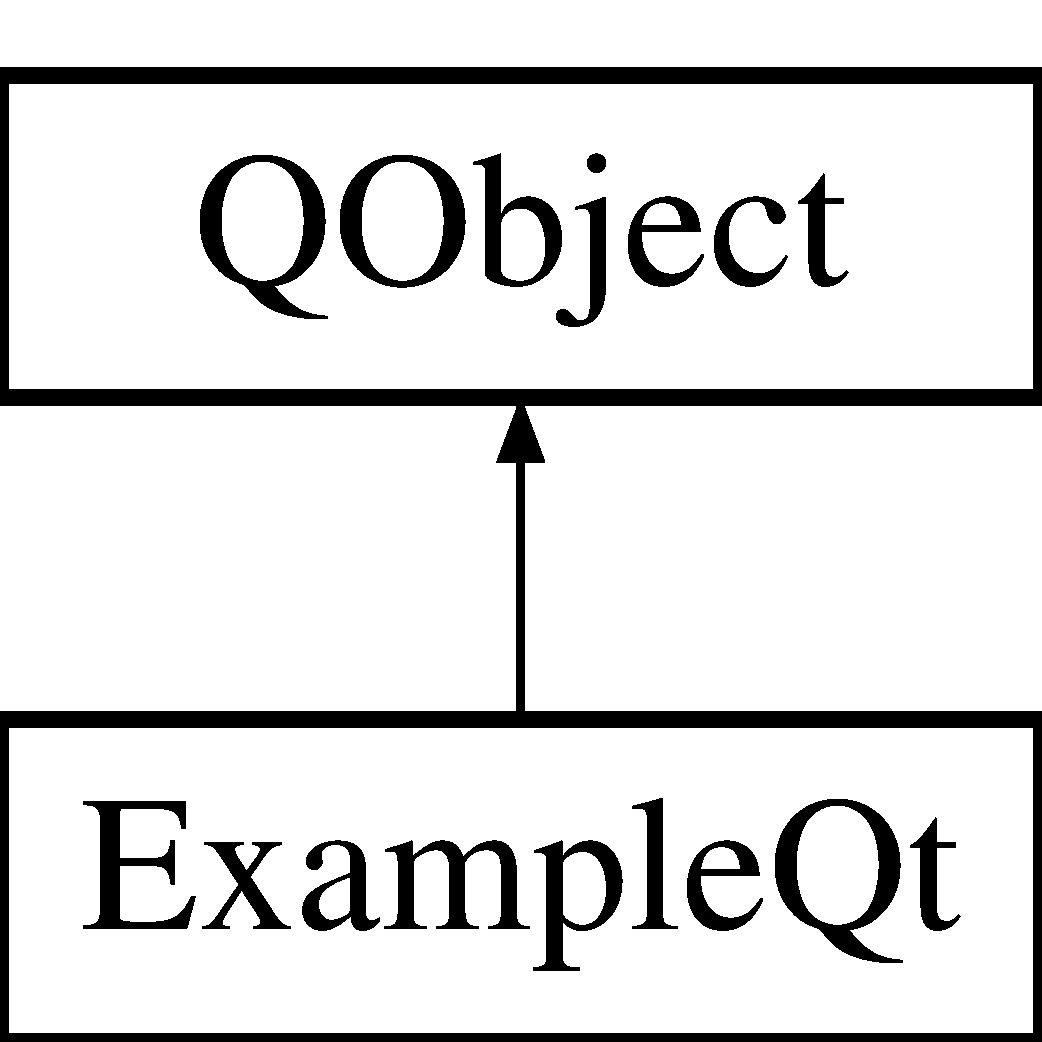
\includegraphics[height=2.000000cm]{class_example_qt}
\end{center}
\end{figure}
\subsection*{Public Slots}
\begin{DoxyCompactItemize}
\item 
\mbox{\Hypertarget{class_example_qt_aa8177d7936135b05c848999600c95e0e}\label{class_example_qt_aa8177d7936135b05c848999600c95e0e}} 
void {\bfseries run} ()
\end{DoxyCompactItemize}
\subsection*{Signals}
\begin{DoxyCompactItemize}
\item 
\mbox{\Hypertarget{class_example_qt_a7d911d1ef947a8ae419cb64f913131a3}\label{class_example_qt_a7d911d1ef947a8ae419cb64f913131a3}} 
void {\bfseries finished} ()
\end{DoxyCompactItemize}
\subsection*{Public Member Functions}
\begin{DoxyCompactItemize}
\item 
\mbox{\Hypertarget{class_example_qt_af45f6ecf229fb42080b290433f1dbdbc}\label{class_example_qt_af45f6ecf229fb42080b290433f1dbdbc}} 
{\bfseries Example\+Qt} (const char $\ast$value, Q\+Object $\ast$parent=0)
\end{DoxyCompactItemize}
\subsection*{Friends}
\begin{DoxyCompactItemize}
\item 
\mbox{\Hypertarget{class_example_qt_a03db4ff40c3001d8f35b6cbc5073a324}\label{class_example_qt_a03db4ff40c3001d8f35b6cbc5073a324}} 
void {\bfseries get\+Callback} (\mbox{\hyperlink{structredis_async_context}{redis\+Async\+Context}} $\ast$, void $\ast$, void $\ast$)
\end{DoxyCompactItemize}


The documentation for this class was generated from the following file\+:\begin{DoxyCompactItemize}
\item 
/\+Users/firatciftci/spellcheck/api/lib/hiredis-\/0.\+13.\+3/examples/example-\/qt.\+h\end{DoxyCompactItemize}

\hypertarget{structmatch__t}{}\section{match\+\_\+t Struct Reference}
\label{structmatch__t}\index{match\+\_\+t@{match\+\_\+t}}
\subsection*{Public Attributes}
\begin{DoxyCompactItemize}
\item 
\mbox{\Hypertarget{structmatch__t_aa66a1f7f9d8d050867ceea0e6ae8e9b9}\label{structmatch__t_aa66a1f7f9d8d050867ceea0e6ae8e9b9}} 
char $\ast$ {\bfseries str}
\item 
\mbox{\Hypertarget{structmatch__t_a7da88d3112f403858d4952f697e5061b}\label{structmatch__t_a7da88d3112f403858d4952f697e5061b}} 
int {\bfseries edits\+\_\+left}
\end{DoxyCompactItemize}


The documentation for this struct was generated from the following file\+:\begin{DoxyCompactItemize}
\item 
/\+Users/firatciftci/spellcheck/api/lib/redis-\/tries/include/suggestion.\+h\end{DoxyCompactItemize}

\hypertarget{structredis_ae_events}{}\section{redis\+Ae\+Events Struct Reference}
\label{structredis_ae_events}\index{redis\+Ae\+Events@{redis\+Ae\+Events}}
\subsection*{Public Attributes}
\begin{DoxyCompactItemize}
\item 
\mbox{\Hypertarget{structredis_ae_events_a8ccdd28fe44a7c4e376a8c8f7cbc0954}\label{structredis_ae_events_a8ccdd28fe44a7c4e376a8c8f7cbc0954}} 
\mbox{\hyperlink{structredis_async_context}{redis\+Async\+Context}} $\ast$ {\bfseries context}
\item 
\mbox{\Hypertarget{structredis_ae_events_abbbedca4a9f5df8e17b39e4bdea83773}\label{structredis_ae_events_abbbedca4a9f5df8e17b39e4bdea83773}} 
ae\+Event\+Loop $\ast$ {\bfseries loop}
\item 
\mbox{\Hypertarget{structredis_ae_events_a0223bf4ebfbf5d32886e06147ea30df1}\label{structredis_ae_events_a0223bf4ebfbf5d32886e06147ea30df1}} 
int {\bfseries fd}
\item 
\mbox{\Hypertarget{structredis_ae_events_abf97765c389403e1c0ee36ac60cd38a5}\label{structredis_ae_events_abf97765c389403e1c0ee36ac60cd38a5}} 
int {\bfseries reading}
\item 
\mbox{\Hypertarget{structredis_ae_events_aef1285c4c876d3c7f4616830d5fc9d3e}\label{structredis_ae_events_aef1285c4c876d3c7f4616830d5fc9d3e}} 
int {\bfseries writing}
\end{DoxyCompactItemize}


The documentation for this struct was generated from the following file\+:\begin{DoxyCompactItemize}
\item 
/\+Users/firatciftci/spellcheck/api/lib/hiredis-\/0.\+13.\+3/adapters/ae.\+h\end{DoxyCompactItemize}

\hypertarget{structredis_async_context}{}\section{redis\+Async\+Context Struct Reference}
\label{structredis_async_context}\index{redis\+Async\+Context@{redis\+Async\+Context}}
\subsection*{Public Attributes}
\begin{DoxyCompactItemize}
\item 
\mbox{\Hypertarget{structredis_async_context_a3c1096341a3041b295c612269394f01b}\label{structredis_async_context_a3c1096341a3041b295c612269394f01b}} 
\mbox{\hyperlink{structredis_context}{redis\+Context}} {\bfseries c}
\item 
\mbox{\Hypertarget{structredis_async_context_a0031ee5988e9a7e827dd1f15baad1d60}\label{structredis_async_context_a0031ee5988e9a7e827dd1f15baad1d60}} 
int {\bfseries err}
\item 
\mbox{\Hypertarget{structredis_async_context_ac8b7a551b88583b36e943a717d4244fc}\label{structredis_async_context_ac8b7a551b88583b36e943a717d4244fc}} 
char $\ast$ {\bfseries errstr}
\item 
\mbox{\Hypertarget{structredis_async_context_a11524847be44957259ec5f8a6c73e832}\label{structredis_async_context_a11524847be44957259ec5f8a6c73e832}} 
void $\ast$ {\bfseries data}
\item 
\mbox{\Hypertarget{structredis_async_context_af44bb2fe80c05bad638d1030ae7c3974}\label{structredis_async_context_af44bb2fe80c05bad638d1030ae7c3974}} 
\begin{tabbing}
xx\=xx\=xx\=xx\=xx\=xx\=xx\=xx\=xx\=\kill
struct \{\\
\>void $\ast$ {\bfseries data}\\
\>void($\ast$ {\bfseries addRead} )(void $\ast$privdata)\\
\>void($\ast$ {\bfseries delRead} )(void $\ast$privdata)\\
\>void($\ast$ {\bfseries addWrite} )(void $\ast$privdata)\\
\>void($\ast$ {\bfseries delWrite} )(void $\ast$privdata)\\
\>void($\ast$ {\bfseries cleanup} )(void $\ast$privdata)\\
\} {\bfseries ev}\\

\end{tabbing}\item 
\mbox{\Hypertarget{structredis_async_context_a3abb6dd544cd420a5fbe8ade6804a2f9}\label{structredis_async_context_a3abb6dd544cd420a5fbe8ade6804a2f9}} 
redis\+Disconnect\+Callback $\ast$ {\bfseries on\+Disconnect}
\item 
\mbox{\Hypertarget{structredis_async_context_a3dc5b4a36a035586e27fd22e5b831da0}\label{structredis_async_context_a3dc5b4a36a035586e27fd22e5b831da0}} 
redis\+Connect\+Callback $\ast$ {\bfseries on\+Connect}
\item 
\mbox{\Hypertarget{structredis_async_context_afa8e9602732ae9746b749db0c0eb366f}\label{structredis_async_context_afa8e9602732ae9746b749db0c0eb366f}} 
\mbox{\hyperlink{structredis_callback_list}{redis\+Callback\+List}} {\bfseries replies}
\item 
\mbox{\Hypertarget{structredis_async_context_aa9151c064088d88cc69410a9e33f93f4}\label{structredis_async_context_aa9151c064088d88cc69410a9e33f93f4}} 
\begin{tabbing}
xx\=xx\=xx\=xx\=xx\=xx\=xx\=xx\=xx\=\kill
struct \{\\
\>\mbox{\hyperlink{structredis_callback_list}{redisCallbackList}} {\bfseries invalid}\\
\>struct \mbox{\hyperlink{structdict}{dict}} $\ast$ {\bfseries channels}\\
\>struct \mbox{\hyperlink{structdict}{dict}} $\ast$ {\bfseries patterns}\\
\} {\bfseries sub}\\

\end{tabbing}\end{DoxyCompactItemize}


The documentation for this struct was generated from the following file\+:\begin{DoxyCompactItemize}
\item 
/\+Users/firatciftci/spellcheck/api/lib/hiredis-\/0.\+13.\+3/async.\+h\end{DoxyCompactItemize}

\hypertarget{structredis_callback}{}\section{redis\+Callback Struct Reference}
\label{structredis_callback}\index{redis\+Callback@{redis\+Callback}}
\subsection*{Public Attributes}
\begin{DoxyCompactItemize}
\item 
\mbox{\Hypertarget{structredis_callback_a36a17df8e50227108adb39ebb7f1a30e}\label{structredis_callback_a36a17df8e50227108adb39ebb7f1a30e}} 
struct \mbox{\hyperlink{structredis_callback}{redis\+Callback}} $\ast$ {\bfseries next}
\item 
\mbox{\Hypertarget{structredis_callback_a2f1bf051a5288a92a21eae88c388d620}\label{structredis_callback_a2f1bf051a5288a92a21eae88c388d620}} 
redis\+Callback\+Fn $\ast$ {\bfseries fn}
\item 
\mbox{\Hypertarget{structredis_callback_ac7c635c7a1a0b69300602b0fddd49a15}\label{structredis_callback_ac7c635c7a1a0b69300602b0fddd49a15}} 
void $\ast$ {\bfseries privdata}
\end{DoxyCompactItemize}


The documentation for this struct was generated from the following file\+:\begin{DoxyCompactItemize}
\item 
/\+Users/firatciftci/spellcheck/api/lib/hiredis-\/0.\+13.\+3/async.\+h\end{DoxyCompactItemize}

\hypertarget{structredis_callback_list}{}\section{redis\+Callback\+List Struct Reference}
\label{structredis_callback_list}\index{redis\+Callback\+List@{redis\+Callback\+List}}
\subsection*{Public Attributes}
\begin{DoxyCompactItemize}
\item 
\mbox{\Hypertarget{structredis_callback_list_aaa0d44375e588947eddbf6745c855cfa}\label{structredis_callback_list_aaa0d44375e588947eddbf6745c855cfa}} 
\mbox{\hyperlink{structredis_callback}{redis\+Callback}} $\ast$ {\bfseries head}
\item 
\mbox{\Hypertarget{structredis_callback_list_ae2b4f074228f4284118df9814135c3bf}\label{structredis_callback_list_ae2b4f074228f4284118df9814135c3bf}} 
\mbox{\hyperlink{structredis_callback}{redis\+Callback}} $\ast$ {\bfseries tail}
\end{DoxyCompactItemize}


The documentation for this struct was generated from the following file\+:\begin{DoxyCompactItemize}
\item 
/\+Users/firatciftci/spellcheck/api/lib/hiredis-\/0.\+13.\+3/async.\+h\end{DoxyCompactItemize}

\hypertarget{structredis_context}{}\section{redis\+Context Struct Reference}
\label{structredis_context}\index{redis\+Context@{redis\+Context}}
\subsection*{Public Attributes}
\begin{DoxyCompactItemize}
\item 
\mbox{\Hypertarget{structredis_context_a481fce8ff0dcee335303d1422ec95444}\label{structredis_context_a481fce8ff0dcee335303d1422ec95444}} 
int {\bfseries err}
\item 
\mbox{\Hypertarget{structredis_context_ace3136a9fe419c796e14fab570eac9c4}\label{structredis_context_ace3136a9fe419c796e14fab570eac9c4}} 
char {\bfseries errstr} \mbox{[}128\mbox{]}
\item 
\mbox{\Hypertarget{structredis_context_af9a3bb9074cc05736a673fcf2961c2aa}\label{structredis_context_af9a3bb9074cc05736a673fcf2961c2aa}} 
int {\bfseries fd}
\item 
\mbox{\Hypertarget{structredis_context_aafd5c9d13dadbd055a8b9607cfd2ee81}\label{structredis_context_aafd5c9d13dadbd055a8b9607cfd2ee81}} 
int {\bfseries flags}
\item 
\mbox{\Hypertarget{structredis_context_a8cab702896e62569c6e44add76157579}\label{structredis_context_a8cab702896e62569c6e44add76157579}} 
char $\ast$ {\bfseries obuf}
\item 
\mbox{\Hypertarget{structredis_context_aae7381e81e013938a73d661eab41f699}\label{structredis_context_aae7381e81e013938a73d661eab41f699}} 
\mbox{\hyperlink{structredis_reader}{redis\+Reader}} $\ast$ {\bfseries reader}
\item 
\mbox{\Hypertarget{structredis_context_ae7324da0f5ca2e9f5d64db2cffd607dc}\label{structredis_context_ae7324da0f5ca2e9f5d64db2cffd607dc}} 
enum redis\+Connection\+Type {\bfseries connection\+\_\+type}
\item 
\mbox{\Hypertarget{structredis_context_a9269266b4f459b0e0dc7603a4bd946fb}\label{structredis_context_a9269266b4f459b0e0dc7603a4bd946fb}} 
struct timeval $\ast$ {\bfseries timeout}
\item 
\mbox{\Hypertarget{structredis_context_a2cd43e1943e302bb818908c9bd6bd633}\label{structredis_context_a2cd43e1943e302bb818908c9bd6bd633}} 
\begin{tabbing}
xx\=xx\=xx\=xx\=xx\=xx\=xx\=xx\=xx\=\kill
struct \{\\
\>char $\ast$ {\bfseries host}\\
\>char $\ast$ {\bfseries source\_addr}\\
\>int {\bfseries port}\\
\} {\bfseries tcp}\\

\end{tabbing}\item 
\mbox{\Hypertarget{structredis_context_aff2d9fc1e4dc37ac4d5aa0d743a05843}\label{structredis_context_aff2d9fc1e4dc37ac4d5aa0d743a05843}} 
\begin{tabbing}
xx\=xx\=xx\=xx\=xx\=xx\=xx\=xx\=xx\=\kill
struct \{\\
\>char $\ast$ {\bfseries path}\\
\} {\bfseries unix\_sock}\\

\end{tabbing}\end{DoxyCompactItemize}


The documentation for this struct was generated from the following file\+:\begin{DoxyCompactItemize}
\item 
/\+Users/firatciftci/spellcheck/api/lib/hiredis-\/0.\+13.\+3/hiredis.\+h\end{DoxyCompactItemize}

\hypertarget{structredis_ivykis_events}{}\section{redis\+Ivykis\+Events Struct Reference}
\label{structredis_ivykis_events}\index{redis\+Ivykis\+Events@{redis\+Ivykis\+Events}}
\subsection*{Public Attributes}
\begin{DoxyCompactItemize}
\item 
\mbox{\Hypertarget{structredis_ivykis_events_aa86981727117ff22f9037cd83f3bf2a4}\label{structredis_ivykis_events_aa86981727117ff22f9037cd83f3bf2a4}} 
\mbox{\hyperlink{structredis_async_context}{redis\+Async\+Context}} $\ast$ {\bfseries context}
\item 
\mbox{\Hypertarget{structredis_ivykis_events_a61a944c6b4066f0478c7aeab66f1585c}\label{structredis_ivykis_events_a61a944c6b4066f0478c7aeab66f1585c}} 
struct iv\+\_\+fd {\bfseries fd}
\end{DoxyCompactItemize}


The documentation for this struct was generated from the following file\+:\begin{DoxyCompactItemize}
\item 
/\+Users/firatciftci/spellcheck/api/lib/hiredis-\/0.\+13.\+3/adapters/ivykis.\+h\end{DoxyCompactItemize}

\hypertarget{structredis_libevent_events}{}\section{redis\+Libevent\+Events Struct Reference}
\label{structredis_libevent_events}\index{redis\+Libevent\+Events@{redis\+Libevent\+Events}}
\subsection*{Public Attributes}
\begin{DoxyCompactItemize}
\item 
\mbox{\Hypertarget{structredis_libevent_events_aa78b057625085c0c0d47b2b54151fa3e}\label{structredis_libevent_events_aa78b057625085c0c0d47b2b54151fa3e}} 
\mbox{\hyperlink{structredis_async_context}{redis\+Async\+Context}} $\ast$ {\bfseries context}
\item 
\mbox{\Hypertarget{structredis_libevent_events_ad323bfd53bac60e96a84e577b1847a50}\label{structredis_libevent_events_ad323bfd53bac60e96a84e577b1847a50}} 
struct event rev {\bfseries wev}
\end{DoxyCompactItemize}


The documentation for this struct was generated from the following file\+:\begin{DoxyCompactItemize}
\item 
/\+Users/firatciftci/spellcheck/api/lib/hiredis-\/0.\+13.\+3/adapters/libevent.\+h\end{DoxyCompactItemize}

\hypertarget{structredis_libev_events}{}\section{redis\+Libev\+Events Struct Reference}
\label{structredis_libev_events}\index{redis\+Libev\+Events@{redis\+Libev\+Events}}
\subsection*{Public Attributes}
\begin{DoxyCompactItemize}
\item 
\mbox{\Hypertarget{structredis_libev_events_a12a3124353d8ac0373dc98a5b17c8dfa}\label{structredis_libev_events_a12a3124353d8ac0373dc98a5b17c8dfa}} 
\mbox{\hyperlink{structredis_async_context}{redis\+Async\+Context}} $\ast$ {\bfseries context}
\item 
\mbox{\Hypertarget{structredis_libev_events_a1dc7b8707661197bf4fbc6ac1dd09863}\label{structredis_libev_events_a1dc7b8707661197bf4fbc6ac1dd09863}} 
struct ev\+\_\+loop $\ast$ {\bfseries loop}
\item 
\mbox{\Hypertarget{structredis_libev_events_ab1022986503c856751f079b51961b138}\label{structredis_libev_events_ab1022986503c856751f079b51961b138}} 
int {\bfseries reading}
\item 
\mbox{\Hypertarget{structredis_libev_events_aef8f75036cbadd7f5be8bfe68f0acd0b}\label{structredis_libev_events_aef8f75036cbadd7f5be8bfe68f0acd0b}} 
int {\bfseries writing}
\item 
\mbox{\Hypertarget{structredis_libev_events_ad0cd2c0f113825469aeedcbf432f5ba9}\label{structredis_libev_events_ad0cd2c0f113825469aeedcbf432f5ba9}} 
ev\+\_\+io {\bfseries rev}
\item 
\mbox{\Hypertarget{structredis_libev_events_ad5d01dc29a5be94df3d8c92ed1ae68e1}\label{structredis_libev_events_ad5d01dc29a5be94df3d8c92ed1ae68e1}} 
ev\+\_\+io {\bfseries wev}
\end{DoxyCompactItemize}


The documentation for this struct was generated from the following file\+:\begin{DoxyCompactItemize}
\item 
/\+Users/firatciftci/spellcheck/api/lib/hiredis-\/0.\+13.\+3/adapters/libev.\+h\end{DoxyCompactItemize}

\hypertarget{structredis_libuv_events}{}\section{redis\+Libuv\+Events Struct Reference}
\label{structredis_libuv_events}\index{redis\+Libuv\+Events@{redis\+Libuv\+Events}}
\subsection*{Public Attributes}
\begin{DoxyCompactItemize}
\item 
\mbox{\Hypertarget{structredis_libuv_events_a328dc1ba61c651da9e658bce18959fa8}\label{structredis_libuv_events_a328dc1ba61c651da9e658bce18959fa8}} 
\mbox{\hyperlink{structredis_async_context}{redis\+Async\+Context}} $\ast$ {\bfseries context}
\item 
\mbox{\Hypertarget{structredis_libuv_events_a27ac1174695e3b6089233f3094c04e6e}\label{structredis_libuv_events_a27ac1174695e3b6089233f3094c04e6e}} 
uv\+\_\+poll\+\_\+t {\bfseries handle}
\item 
\mbox{\Hypertarget{structredis_libuv_events_ae1c36a588f0f5c27c2244673532457aa}\label{structredis_libuv_events_ae1c36a588f0f5c27c2244673532457aa}} 
int {\bfseries events}
\end{DoxyCompactItemize}


The documentation for this struct was generated from the following file\+:\begin{DoxyCompactItemize}
\item 
/\+Users/firatciftci/spellcheck/api/lib/hiredis-\/0.\+13.\+3/adapters/libuv.\+h\end{DoxyCompactItemize}

\hypertarget{class_redis_qt_adapter}{}\section{Redis\+Qt\+Adapter Class Reference}
\label{class_redis_qt_adapter}\index{Redis\+Qt\+Adapter@{Redis\+Qt\+Adapter}}
Inheritance diagram for Redis\+Qt\+Adapter\+:\begin{figure}[H]
\begin{center}
\leavevmode
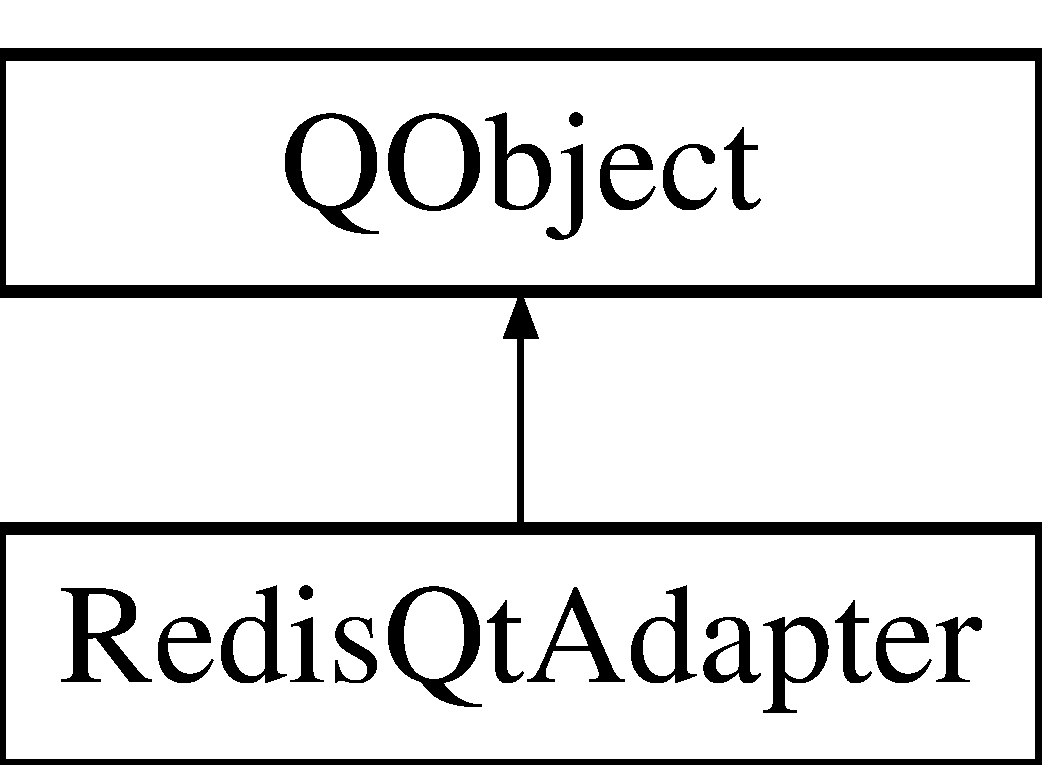
\includegraphics[height=2.000000cm]{class_redis_qt_adapter}
\end{center}
\end{figure}
\subsection*{Public Member Functions}
\begin{DoxyCompactItemize}
\item 
\mbox{\Hypertarget{class_redis_qt_adapter_a81ea7cccc1ee7630afc739c20fecf868}\label{class_redis_qt_adapter_a81ea7cccc1ee7630afc739c20fecf868}} 
{\bfseries Redis\+Qt\+Adapter} (Q\+Object $\ast$parent=0)
\item 
\mbox{\Hypertarget{class_redis_qt_adapter_a7189a89d981e7c8b7a6de68ae1972bee}\label{class_redis_qt_adapter_a7189a89d981e7c8b7a6de68ae1972bee}} 
int {\bfseries set\+Context} (\mbox{\hyperlink{structredis_async_context}{redis\+Async\+Context}} $\ast$ac)
\end{DoxyCompactItemize}
\subsection*{Friends}
\begin{DoxyCompactItemize}
\item 
\mbox{\Hypertarget{class_redis_qt_adapter_ac409536f14d25acb71bdf215d9011d41}\label{class_redis_qt_adapter_ac409536f14d25acb71bdf215d9011d41}} 
void {\bfseries Redis\+Qt\+Add\+Read} (void $\ast$adapter)
\item 
\mbox{\Hypertarget{class_redis_qt_adapter_a1d82512957df3da1367ef6512c713ac1}\label{class_redis_qt_adapter_a1d82512957df3da1367ef6512c713ac1}} 
void {\bfseries Redis\+Qt\+Del\+Read} (void $\ast$adapter)
\item 
\mbox{\Hypertarget{class_redis_qt_adapter_a9784ddb1261db4538070de4ce75aa8d7}\label{class_redis_qt_adapter_a9784ddb1261db4538070de4ce75aa8d7}} 
void {\bfseries Redis\+Qt\+Add\+Write} (void $\ast$adapter)
\item 
\mbox{\Hypertarget{class_redis_qt_adapter_ab17cffda634d28ce2e0467ca8c1e0666}\label{class_redis_qt_adapter_ab17cffda634d28ce2e0467ca8c1e0666}} 
void {\bfseries Redis\+Qt\+Del\+Write} (void $\ast$adapter)
\item 
\mbox{\Hypertarget{class_redis_qt_adapter_ab4f4f4eab9c4a9d4209c9869859412b4}\label{class_redis_qt_adapter_ab4f4f4eab9c4a9d4209c9869859412b4}} 
void {\bfseries Redis\+Qt\+Cleanup} (void $\ast$adapter)
\end{DoxyCompactItemize}


The documentation for this class was generated from the following file\+:\begin{DoxyCompactItemize}
\item 
/\+Users/firatciftci/spellcheck/api/lib/hiredis-\/0.\+13.\+3/adapters/qt.\+h\end{DoxyCompactItemize}

\hypertarget{structredis_reader}{}\section{redis\+Reader Struct Reference}
\label{structredis_reader}\index{redis\+Reader@{redis\+Reader}}
\subsection*{Public Attributes}
\begin{DoxyCompactItemize}
\item 
\mbox{\Hypertarget{structredis_reader_ad579da9500bb3f8c97b79ed4f8c24805}\label{structredis_reader_ad579da9500bb3f8c97b79ed4f8c24805}} 
int {\bfseries err}
\item 
\mbox{\Hypertarget{structredis_reader_a7af28e9c4e7a4c1ccd8cf8eefb277615}\label{structredis_reader_a7af28e9c4e7a4c1ccd8cf8eefb277615}} 
char {\bfseries errstr} \mbox{[}128\mbox{]}
\item 
\mbox{\Hypertarget{structredis_reader_a2f15e6a06fde31acc1765e22776e5a24}\label{structredis_reader_a2f15e6a06fde31acc1765e22776e5a24}} 
char $\ast$ {\bfseries buf}
\item 
\mbox{\Hypertarget{structredis_reader_af57fca3220a12be68ddb2e8001d21485}\label{structredis_reader_af57fca3220a12be68ddb2e8001d21485}} 
size\+\_\+t {\bfseries pos}
\item 
\mbox{\Hypertarget{structredis_reader_ac16e7c62f35a4f303d61647e6afa9512}\label{structredis_reader_ac16e7c62f35a4f303d61647e6afa9512}} 
size\+\_\+t {\bfseries len}
\item 
\mbox{\Hypertarget{structredis_reader_ae90fdd33997ad3933dc81fea34e7a012}\label{structredis_reader_ae90fdd33997ad3933dc81fea34e7a012}} 
size\+\_\+t {\bfseries maxbuf}
\item 
\mbox{\Hypertarget{structredis_reader_a080b2b270dcc6362f8c8f974d42be9f7}\label{structredis_reader_a080b2b270dcc6362f8c8f974d42be9f7}} 
\mbox{\hyperlink{structredis_read_task}{redis\+Read\+Task}} {\bfseries rstack} \mbox{[}9\mbox{]}
\item 
\mbox{\Hypertarget{structredis_reader_a5d8453b01f50ecad257d26b2b322b9a0}\label{structredis_reader_a5d8453b01f50ecad257d26b2b322b9a0}} 
int {\bfseries ridx}
\item 
\mbox{\Hypertarget{structredis_reader_aa2684486789472eee6e88723b06a4335}\label{structredis_reader_aa2684486789472eee6e88723b06a4335}} 
void $\ast$ {\bfseries reply}
\item 
\mbox{\Hypertarget{structredis_reader_aef207ed70dcbd6c9ac9071d40c8becb2}\label{structredis_reader_aef207ed70dcbd6c9ac9071d40c8becb2}} 
\mbox{\hyperlink{structredis_reply_object_functions}{redis\+Reply\+Object\+Functions}} $\ast$ {\bfseries fn}
\item 
\mbox{\Hypertarget{structredis_reader_a26d3b75a46555f9836849e160bc0b6de}\label{structredis_reader_a26d3b75a46555f9836849e160bc0b6de}} 
void $\ast$ {\bfseries privdata}
\end{DoxyCompactItemize}


The documentation for this struct was generated from the following file\+:\begin{DoxyCompactItemize}
\item 
/\+Users/firatciftci/spellcheck/api/lib/hiredis-\/0.\+13.\+3/read.\+h\end{DoxyCompactItemize}

\hypertarget{structredis_read_task}{}\section{redis\+Read\+Task Struct Reference}
\label{structredis_read_task}\index{redis\+Read\+Task@{redis\+Read\+Task}}
\subsection*{Public Attributes}
\begin{DoxyCompactItemize}
\item 
\mbox{\Hypertarget{structredis_read_task_a5d4a4d7982388a9e4279a29992347701}\label{structredis_read_task_a5d4a4d7982388a9e4279a29992347701}} 
int {\bfseries type}
\item 
\mbox{\Hypertarget{structredis_read_task_a05d573c401dfa561dadcf3d7fab12240}\label{structredis_read_task_a05d573c401dfa561dadcf3d7fab12240}} 
int {\bfseries elements}
\item 
\mbox{\Hypertarget{structredis_read_task_ad2b467d141591945b8ae2fa15a8149c1}\label{structredis_read_task_ad2b467d141591945b8ae2fa15a8149c1}} 
int {\bfseries idx}
\item 
\mbox{\Hypertarget{structredis_read_task_a7c29675175129f56c513effb756a8ac8}\label{structredis_read_task_a7c29675175129f56c513effb756a8ac8}} 
void $\ast$ {\bfseries obj}
\item 
\mbox{\Hypertarget{structredis_read_task_a8ca682f575a18cae9207a81e3c10db1d}\label{structredis_read_task_a8ca682f575a18cae9207a81e3c10db1d}} 
struct \mbox{\hyperlink{structredis_read_task}{redis\+Read\+Task}} $\ast$ {\bfseries parent}
\item 
\mbox{\Hypertarget{structredis_read_task_af98c4f81471ba383dde5e89fdbceedaa}\label{structredis_read_task_af98c4f81471ba383dde5e89fdbceedaa}} 
void $\ast$ {\bfseries privdata}
\end{DoxyCompactItemize}


The documentation for this struct was generated from the following file\+:\begin{DoxyCompactItemize}
\item 
/\+Users/firatciftci/spellcheck/api/lib/hiredis-\/0.\+13.\+3/read.\+h\end{DoxyCompactItemize}

\hypertarget{structredis_reply}{}\section{redis\+Reply Struct Reference}
\label{structredis_reply}\index{redis\+Reply@{redis\+Reply}}
\subsection*{Public Attributes}
\begin{DoxyCompactItemize}
\item 
\mbox{\Hypertarget{structredis_reply_ae0f63252174a354d1c2d6166ca1561a7}\label{structredis_reply_ae0f63252174a354d1c2d6166ca1561a7}} 
int {\bfseries type}
\item 
\mbox{\Hypertarget{structredis_reply_afeea337ee0f85106d6b5bc78d1ed7e0a}\label{structredis_reply_afeea337ee0f85106d6b5bc78d1ed7e0a}} 
long long {\bfseries integer}
\item 
\mbox{\Hypertarget{structredis_reply_aee07b9671e698a7f36d4ef72d27ca47e}\label{structredis_reply_aee07b9671e698a7f36d4ef72d27ca47e}} 
int {\bfseries len}
\item 
\mbox{\Hypertarget{structredis_reply_a3f90c90562204a5a44bde464c12c7d44}\label{structredis_reply_a3f90c90562204a5a44bde464c12c7d44}} 
char $\ast$ {\bfseries str}
\item 
\mbox{\Hypertarget{structredis_reply_a5d119457290bdb62236b59480a45a7b7}\label{structredis_reply_a5d119457290bdb62236b59480a45a7b7}} 
size\+\_\+t {\bfseries elements}
\item 
\mbox{\Hypertarget{structredis_reply_abeda65603c39ad7aeeae9c647dd99d1e}\label{structredis_reply_abeda65603c39ad7aeeae9c647dd99d1e}} 
struct \mbox{\hyperlink{structredis_reply}{redis\+Reply}} $\ast$$\ast$ {\bfseries element}
\end{DoxyCompactItemize}


The documentation for this struct was generated from the following file\+:\begin{DoxyCompactItemize}
\item 
/\+Users/firatciftci/spellcheck/api/lib/hiredis-\/0.\+13.\+3/hiredis.\+h\end{DoxyCompactItemize}

\hypertarget{structredis_reply_object_functions}{}\section{redis\+Reply\+Object\+Functions Struct Reference}
\label{structredis_reply_object_functions}\index{redis\+Reply\+Object\+Functions@{redis\+Reply\+Object\+Functions}}
\subsection*{Public Attributes}
\begin{DoxyCompactItemize}
\item 
\mbox{\Hypertarget{structredis_reply_object_functions_aaee312b4a7cb8cffc0c7a588dd3066ec}\label{structredis_reply_object_functions_aaee312b4a7cb8cffc0c7a588dd3066ec}} 
void $\ast$($\ast$ {\bfseries create\+String} )(const \mbox{\hyperlink{structredis_read_task}{redis\+Read\+Task}} $\ast$, char $\ast$, size\+\_\+t)
\item 
\mbox{\Hypertarget{structredis_reply_object_functions_aeb36b84075f737cce48f6da24dc863fa}\label{structredis_reply_object_functions_aeb36b84075f737cce48f6da24dc863fa}} 
void $\ast$($\ast$ {\bfseries create\+Array} )(const \mbox{\hyperlink{structredis_read_task}{redis\+Read\+Task}} $\ast$, int)
\item 
\mbox{\Hypertarget{structredis_reply_object_functions_abd65f8490555ca7b36e8b3e5174e06cf}\label{structredis_reply_object_functions_abd65f8490555ca7b36e8b3e5174e06cf}} 
void $\ast$($\ast$ {\bfseries create\+Integer} )(const \mbox{\hyperlink{structredis_read_task}{redis\+Read\+Task}} $\ast$, long long)
\item 
\mbox{\Hypertarget{structredis_reply_object_functions_a7dd9fb4c1e6df6c9b552513c768d74dd}\label{structredis_reply_object_functions_a7dd9fb4c1e6df6c9b552513c768d74dd}} 
void $\ast$($\ast$ {\bfseries create\+Nil} )(const \mbox{\hyperlink{structredis_read_task}{redis\+Read\+Task}} $\ast$)
\item 
\mbox{\Hypertarget{structredis_reply_object_functions_a3fbe4633d7a5447a8809f538b6ffd569}\label{structredis_reply_object_functions_a3fbe4633d7a5447a8809f538b6ffd569}} 
void($\ast$ {\bfseries free\+Object} )(void $\ast$)
\end{DoxyCompactItemize}


The documentation for this struct was generated from the following file\+:\begin{DoxyCompactItemize}
\item 
/\+Users/firatciftci/spellcheck/api/lib/hiredis-\/0.\+13.\+3/read.\+h\end{DoxyCompactItemize}

\hypertarget{struct_redis_run_loop}{}\section{Redis\+Run\+Loop Struct Reference}
\label{struct_redis_run_loop}\index{Redis\+Run\+Loop@{Redis\+Run\+Loop}}
\subsection*{Public Attributes}
\begin{DoxyCompactItemize}
\item 
\mbox{\Hypertarget{struct_redis_run_loop_a082be18e46a6b0bba89f9b6a7c44545d}\label{struct_redis_run_loop_a082be18e46a6b0bba89f9b6a7c44545d}} 
\mbox{\hyperlink{structredis_async_context}{redis\+Async\+Context}} $\ast$ {\bfseries context}
\item 
\mbox{\Hypertarget{struct_redis_run_loop_aaec03e51273ef0e0d76778d2078c4674}\label{struct_redis_run_loop_aaec03e51273ef0e0d76778d2078c4674}} 
C\+F\+Socket\+Ref {\bfseries socket\+Ref}
\item 
\mbox{\Hypertarget{struct_redis_run_loop_a5083e4a92d5ba2821343b9ff170ccc3b}\label{struct_redis_run_loop_a5083e4a92d5ba2821343b9ff170ccc3b}} 
C\+F\+Run\+Loop\+Source\+Ref {\bfseries source\+Ref}
\end{DoxyCompactItemize}


The documentation for this struct was generated from the following file\+:\begin{DoxyCompactItemize}
\item 
/\+Users/firatciftci/spellcheck/api/lib/hiredis-\/0.\+13.\+3/adapters/macosx.\+h\end{DoxyCompactItemize}

\hypertarget{struct_redis_source}{}\section{Redis\+Source Struct Reference}
\label{struct_redis_source}\index{Redis\+Source@{Redis\+Source}}
\subsection*{Public Attributes}
\begin{DoxyCompactItemize}
\item 
\mbox{\Hypertarget{struct_redis_source_a524fa1a913774c654158eeaaa1ef2646}\label{struct_redis_source_a524fa1a913774c654158eeaaa1ef2646}} 
G\+Source {\bfseries source}
\item 
\mbox{\Hypertarget{struct_redis_source_accf3950d2f35a039f3dce9b07995b63e}\label{struct_redis_source_accf3950d2f35a039f3dce9b07995b63e}} 
\mbox{\hyperlink{structredis_async_context}{redis\+Async\+Context}} $\ast$ {\bfseries ac}
\item 
\mbox{\Hypertarget{struct_redis_source_a0cd8eea6b8310910d9bdf866f8882377}\label{struct_redis_source_a0cd8eea6b8310910d9bdf866f8882377}} 
G\+Poll\+FD {\bfseries poll\+\_\+fd}
\end{DoxyCompactItemize}


The documentation for this struct was generated from the following file\+:\begin{DoxyCompactItemize}
\item 
/\+Users/firatciftci/spellcheck/api/lib/hiredis-\/0.\+13.\+3/adapters/glib.\+h\end{DoxyCompactItemize}

\hypertarget{structsdshdr}{}\section{sdshdr Struct Reference}
\label{structsdshdr}\index{sdshdr@{sdshdr}}
\subsection*{Public Attributes}
\begin{DoxyCompactItemize}
\item 
\mbox{\Hypertarget{structsdshdr_a6550b193c38a86423fcfb1b14779b117}\label{structsdshdr_a6550b193c38a86423fcfb1b14779b117}} 
int {\bfseries len}
\item 
\mbox{\Hypertarget{structsdshdr_a37a1284cc7168d3ac6b6fceabad74b8c}\label{structsdshdr_a37a1284cc7168d3ac6b6fceabad74b8c}} 
int {\bfseries free}
\item 
\mbox{\Hypertarget{structsdshdr_af505c8157c3faec30b8e32f0b552fc12}\label{structsdshdr_af505c8157c3faec30b8e32f0b552fc12}} 
char {\bfseries buf} \mbox{[}$\,$\mbox{]}
\end{DoxyCompactItemize}


The documentation for this struct was generated from the following file\+:\begin{DoxyCompactItemize}
\item 
/\+Users/firatciftci/spellcheck/api/lib/hiredis-\/0.\+13.\+3/sds.\+h\end{DoxyCompactItemize}

\hypertarget{structtrie}{}\section{trie Struct Reference}
\label{structtrie}\index{trie@{trie}}
\subsection*{Public Attributes}
\begin{DoxyCompactItemize}
\item 
\mbox{\Hypertarget{structtrie_ae0b1f0e70e6499cf5b37e2322e30d16c}\label{structtrie_ae0b1f0e70e6499cf5b37e2322e30d16c}} 
char {\bfseries current}
\item 
\mbox{\Hypertarget{structtrie_aef4d5c101069c280c08ed23636505079}\label{structtrie_aef4d5c101069c280c08ed23636505079}} 
struct \mbox{\hyperlink{structtrie}{trie}} $\ast$$\ast$ {\bfseries children}
\item 
\mbox{\Hypertarget{structtrie_a1aad2f91026a96305ca9489eea8c5720}\label{structtrie_a1aad2f91026a96305ca9489eea8c5720}} 
int {\bfseries is\+\_\+word}
\item 
\mbox{\Hypertarget{structtrie_a5623bbbf793b4659b2badfadae983034}\label{structtrie_a5623bbbf793b4659b2badfadae983034}} 
struct \mbox{\hyperlink{structtrie}{trie}} $\ast$ {\bfseries parent}
\item 
\mbox{\Hypertarget{structtrie_af4a9ad62a2178649f867d1ed52af2ca6}\label{structtrie_af4a9ad62a2178649f867d1ed52af2ca6}} 
char $\ast$ {\bfseries charlist}
\end{DoxyCompactItemize}


The documentation for this struct was generated from the following file\+:\begin{DoxyCompactItemize}
\item 
/\+Users/firatciftci/spellcheck/api/lib/redis-\/tries/module/trie.\+c\end{DoxyCompactItemize}

\hypertarget{structtrie__t}{}\section{trie\+\_\+t Struct Reference}
\label{structtrie__t}\index{trie\+\_\+t@{trie\+\_\+t}}
\subsection*{Public Attributes}
\begin{DoxyCompactItemize}
\item 
\mbox{\Hypertarget{structtrie__t_a0be3fb3ebf84d9885bcaa68441d3cab8}\label{structtrie__t_a0be3fb3ebf84d9885bcaa68441d3cab8}} 
char $\ast$ {\bfseries name}
\item 
\mbox{\Hypertarget{structtrie__t_a25e213993060741a97775472ec4b310b}\label{structtrie__t_a25e213993060741a97775472ec4b310b}} 
\mbox{\hyperlink{structredis_context}{redis\+Context}} $\ast$ {\bfseries context}
\item 
\mbox{\Hypertarget{structtrie__t_a9b6d9cd7d752c92d3b326e1efc4151d8}\label{structtrie__t_a9b6d9cd7d752c92d3b326e1efc4151d8}} 
char {\bfseries current}
\item 
\mbox{\Hypertarget{structtrie__t_af1cba62258760e7873144bbfec433b4a}\label{structtrie__t_af1cba62258760e7873144bbfec433b4a}} 
\mbox{\hyperlink{structtrie__t}{trie\+\_\+t}} $\ast$$\ast$ {\bfseries children}
\item 
\mbox{\Hypertarget{structtrie__t_afcc58db1561cb97ab235d72d10718522}\label{structtrie__t_afcc58db1561cb97ab235d72d10718522}} 
int {\bfseries is\+\_\+word}
\item 
\mbox{\Hypertarget{structtrie__t_a258d66a0e141a22cd12547e0b2fc6d69}\label{structtrie__t_a258d66a0e141a22cd12547e0b2fc6d69}} 
\mbox{\hyperlink{structtrie__t}{trie\+\_\+t}} $\ast$ {\bfseries parent}
\item 
\mbox{\Hypertarget{structtrie__t_a2707a8b13123d8109d0540e1383d6604}\label{structtrie__t_a2707a8b13123d8109d0540e1383d6604}} 
char $\ast$ {\bfseries charlist}
\end{DoxyCompactItemize}


The documentation for this struct was generated from the following file\+:\begin{DoxyCompactItemize}
\item 
/\+Users/firatciftci/spellcheck/api/include/trie.\+h\end{DoxyCompactItemize}

\hypertarget{structzset__t}{}\section{zset\+\_\+t Struct Reference}
\label{structzset__t}\index{zset\+\_\+t@{zset\+\_\+t}}
\subsection*{Public Attributes}
\begin{DoxyCompactItemize}
\item 
\mbox{\Hypertarget{structzset__t_aac0cee826c38fc2cafc1b12767970fe1}\label{structzset__t_aac0cee826c38fc2cafc1b12767970fe1}} 
char $\ast$ {\bfseries name}
\item 
\mbox{\Hypertarget{structzset__t_aa63f9f702c85919482a586095182e13f}\label{structzset__t_aa63f9f702c85919482a586095182e13f}} 
\mbox{\hyperlink{structredis_context}{redis\+Context}} $\ast$ {\bfseries context}
\end{DoxyCompactItemize}


The documentation for this struct was generated from the following file\+:\begin{DoxyCompactItemize}
\item 
/\+Users/firatciftci/spellcheck/api/include/zset.\+h\end{DoxyCompactItemize}

\chapter{File Documentation}
\hypertarget{shellstrings_8h}{}\section{/\+Users/jaewanpark/\+Desktop/\+V\+M\+\_\+\+R\+E\+P\+O\+\_\+\+R\+O\+O\+T/spellcheck/include/shellstrings.h File Reference}
\label{shellstrings_8h}\index{/\+Users/jaewanpark/\+Desktop/\+V\+M\+\_\+\+R\+E\+P\+O\+\_\+\+R\+O\+O\+T/spellcheck/include/shellstrings.\+h@{/\+Users/jaewanpark/\+Desktop/\+V\+M\+\_\+\+R\+E\+P\+O\+\_\+\+R\+O\+O\+T/spellcheck/include/shellstrings.\+h}}
{\ttfamily \#include $<$stdio.\+h$>$}\newline
{\ttfamily \#include $<$stdlib.\+h$>$}\newline
{\ttfamily \#include $<$stdbool.\+h$>$}\newline
{\ttfamily \#include $<$string.\+h$>$}\newline
\subsection*{Macros}
\begin{DoxyCompactItemize}
\item 
\mbox{\Hypertarget{shellstrings_8h_ab702106cf3b3e96750b6845ded4e0299}\label{shellstrings_8h_ab702106cf3b3e96750b6845ded4e0299}} 
\#define \mbox{\hyperlink{shellstrings_8h_ab702106cf3b3e96750b6845ded4e0299}{R\+E\+S\+ET}}~\char`\"{}\textbackslash{}033\mbox{[}0m\char`\"{}
\begin{DoxyCompactList}\small\item\em Resets printf() color to white. \end{DoxyCompactList}\item 
\mbox{\Hypertarget{shellstrings_8h_a8d23feea868a983c8c2b661e1e16972f}\label{shellstrings_8h_a8d23feea868a983c8c2b661e1e16972f}} 
\#define \mbox{\hyperlink{shellstrings_8h_a8d23feea868a983c8c2b661e1e16972f}{R\+ED}}~\char`\"{}\textbackslash{}033\mbox{[}31m\char`\"{}
\begin{DoxyCompactList}\small\item\em Changes printf() color to red. \end{DoxyCompactList}\item 
\mbox{\Hypertarget{shellstrings_8h_abf681265909adf3d3e8116c93c0ba179}\label{shellstrings_8h_abf681265909adf3d3e8116c93c0ba179}} 
\#define \mbox{\hyperlink{shellstrings_8h_abf681265909adf3d3e8116c93c0ba179}{Y\+E\+L\+L\+OW}}~\char`\"{}\textbackslash{}033\mbox{[}33m\char`\"{}
\begin{DoxyCompactList}\small\item\em Changes printf() color to yellow. \end{DoxyCompactList}\item 
\mbox{\Hypertarget{shellstrings_8h_a79d10e672abb49ad63eeaa8aaef57c38}\label{shellstrings_8h_a79d10e672abb49ad63eeaa8aaef57c38}} 
\#define \mbox{\hyperlink{shellstrings_8h_a79d10e672abb49ad63eeaa8aaef57c38}{B\+L\+UE}}~\char`\"{}\textbackslash{}033\mbox{[}34m\char`\"{}
\begin{DoxyCompactList}\small\item\em Changes printf() color to blue. \end{DoxyCompactList}\item 
\mbox{\Hypertarget{shellstrings_8h_acfbc006ea433ad708fdee3e82996e721}\label{shellstrings_8h_acfbc006ea433ad708fdee3e82996e721}} 
\#define \mbox{\hyperlink{shellstrings_8h_acfbc006ea433ad708fdee3e82996e721}{G\+R\+E\+EN}}~\char`\"{}\textbackslash{}033\mbox{[}32m\char`\"{}
\begin{DoxyCompactList}\small\item\em Changes printf() color to green. \end{DoxyCompactList}\item 
\mbox{\Hypertarget{shellstrings_8h_a87b537f5fa5c109d3c05c13d6b18f382}\label{shellstrings_8h_a87b537f5fa5c109d3c05c13d6b18f382}} 
\#define \mbox{\hyperlink{shellstrings_8h_a87b537f5fa5c109d3c05c13d6b18f382}{W\+H\+I\+TE}}~\char`\"{}\textbackslash{}033\mbox{[}37m\char`\"{}
\begin{DoxyCompactList}\small\item\em Changes printf() color to white. \end{DoxyCompactList}\item 
\mbox{\Hypertarget{shellstrings_8h_ab912d02c7998c3d47d05f87be4e2c920}\label{shellstrings_8h_ab912d02c7998c3d47d05f87be4e2c920}} 
\#define \mbox{\hyperlink{shellstrings_8h_ab912d02c7998c3d47d05f87be4e2c920}{B\+O\+L\+D\+R\+ED}}~\char`\"{}\textbackslash{}033\mbox{[}1m\textbackslash{}033\mbox{[}31m\char`\"{}
\begin{DoxyCompactList}\small\item\em Changes printf() color to bold red. \end{DoxyCompactList}\item 
\mbox{\Hypertarget{shellstrings_8h_a8cec79108dfc3c61e8e32d390ec28b26}\label{shellstrings_8h_a8cec79108dfc3c61e8e32d390ec28b26}} 
\#define \mbox{\hyperlink{shellstrings_8h_a8cec79108dfc3c61e8e32d390ec28b26}{B\+O\+L\+D\+Y\+E\+L\+L\+OW}}~\char`\"{}\textbackslash{}033\mbox{[}1m\textbackslash{}033\mbox{[}33m\char`\"{}
\begin{DoxyCompactList}\small\item\em Changes printf() color to bold yellow. \end{DoxyCompactList}\item 
\mbox{\Hypertarget{shellstrings_8h_a11e77c19555cbd15bcc744ff36a18635}\label{shellstrings_8h_a11e77c19555cbd15bcc744ff36a18635}} 
\#define \mbox{\hyperlink{shellstrings_8h_a11e77c19555cbd15bcc744ff36a18635}{B\+O\+L\+D\+B\+L\+UE}}~\char`\"{}\textbackslash{}033\mbox{[}1m\textbackslash{}033\mbox{[}34m\char`\"{}
\begin{DoxyCompactList}\small\item\em Changes printf() color to bold blue. \end{DoxyCompactList}\item 
\mbox{\Hypertarget{shellstrings_8h_a4a6c893a1703c33ede7d702fe5f97c91}\label{shellstrings_8h_a4a6c893a1703c33ede7d702fe5f97c91}} 
\#define \mbox{\hyperlink{shellstrings_8h_a4a6c893a1703c33ede7d702fe5f97c91}{B\+O\+L\+D\+G\+R\+E\+EN}}~\char`\"{}\textbackslash{}033\mbox{[}1m\textbackslash{}033\mbox{[}32m\char`\"{}
\begin{DoxyCompactList}\small\item\em Changes printf() color to bold green. \end{DoxyCompactList}\item 
\mbox{\Hypertarget{shellstrings_8h_aa4ef051614aa0bd503b0a18ee158c5d7}\label{shellstrings_8h_aa4ef051614aa0bd503b0a18ee158c5d7}} 
\#define \mbox{\hyperlink{shellstrings_8h_aa4ef051614aa0bd503b0a18ee158c5d7}{B\+O\+L\+D\+W\+H\+I\+TE}}~\char`\"{}\textbackslash{}033\mbox{[}1m\textbackslash{}033\mbox{[}37m\char`\"{}
\begin{DoxyCompactList}\small\item\em Changes printf() color to bold white. \end{DoxyCompactList}\end{DoxyCompactItemize}
\subsection*{Functions}
\begin{DoxyCompactItemize}
\item 
void \mbox{\hyperlink{shellstrings_8h_ac04b0924a2f76ada92ce310ffc214e9e}{shell\+\_\+prompt}} (bool color)
\begin{DoxyCompactList}\small\item\em Default text input prompt string for the shell. \end{DoxyCompactList}\item 
void \mbox{\hyperlink{shellstrings_8h_ac62e924043236c64ae2163ccd5d9a3e3}{shell\+\_\+main\+\_\+menu}} (bool color)
\begin{DoxyCompactList}\small\item\em Main menu text for the shell. \end{DoxyCompactList}\end{DoxyCompactItemize}


\subsection{Detailed Description}
String printing library for the shell. 

\subsection{Function Documentation}
\mbox{\Hypertarget{shellstrings_8h_ac62e924043236c64ae2163ccd5d9a3e3}\label{shellstrings_8h_ac62e924043236c64ae2163ccd5d9a3e3}} 
\index{shellstrings.\+h@{shellstrings.\+h}!shell\+\_\+main\+\_\+menu@{shell\+\_\+main\+\_\+menu}}
\index{shell\+\_\+main\+\_\+menu@{shell\+\_\+main\+\_\+menu}!shellstrings.\+h@{shellstrings.\+h}}
\subsubsection{\texorpdfstring{shell\+\_\+main\+\_\+menu()}{shell\_main\_menu()}}
{\footnotesize\ttfamily void shell\+\_\+main\+\_\+menu (\begin{DoxyParamCaption}\item[{bool}]{color }\end{DoxyParamCaption})}



Main menu text for the shell. 


\begin{DoxyParams}{Parameters}
{\em color} & Boolean to enable/disable the color functionality. \\
\hline
\end{DoxyParams}
\mbox{\Hypertarget{shellstrings_8h_ac04b0924a2f76ada92ce310ffc214e9e}\label{shellstrings_8h_ac04b0924a2f76ada92ce310ffc214e9e}} 
\index{shellstrings.\+h@{shellstrings.\+h}!shell\+\_\+prompt@{shell\+\_\+prompt}}
\index{shell\+\_\+prompt@{shell\+\_\+prompt}!shellstrings.\+h@{shellstrings.\+h}}
\subsubsection{\texorpdfstring{shell\+\_\+prompt()}{shell\_prompt()}}
{\footnotesize\ttfamily void shell\+\_\+prompt (\begin{DoxyParamCaption}\item[{bool}]{color }\end{DoxyParamCaption})}



Default text input prompt string for the shell. 


\begin{DoxyParams}{Parameters}
{\em color} & Boolean to enable/disable the color functionality. \\
\hline
\end{DoxyParams}

%--- End generated contents ---

% Index
\backmatter
\newpage
\phantomsection
\clearemptydoublepage
\addcontentsline{toc}{chapter}{\indexname}
\printindex

\end{document}
